\documentclass[1p]{elsarticle_modified}
%\bibliographystyle{elsarticle-num}

%\usepackage[colorlinks]{hyperref}
%\usepackage{abbrmath_seonhwa} %\Abb, \Ascr, \Acal ,\Abf, \Afrak
\usepackage{amsfonts}
\usepackage{amssymb}
\usepackage{amsmath}
\usepackage{amsthm}
\usepackage{scalefnt}
\usepackage{amsbsy}
\usepackage{kotex}
\usepackage{caption}
\usepackage{subfig}
\usepackage{color}
\usepackage{graphicx}
\usepackage{xcolor} %% white, black, red, green, blue, cyan, magenta, yellow
\usepackage{float}
\usepackage{setspace}
\usepackage{hyperref}

\usepackage{tikz}
\usetikzlibrary{arrows}

\usepackage{multirow}
\usepackage{array} % fixed length table
\usepackage{hhline}

%%%%%%%%%%%%%%%%%%%%%
\makeatletter
\renewcommand*\env@matrix[1][\arraystretch]{%
	\edef\arraystretch{#1}%
	\hskip -\arraycolsep
	\let\@ifnextchar\new@ifnextchar
	\array{*\c@MaxMatrixCols c}}
\makeatother %https://tex.stackexchange.com/questions/14071/how-can-i-increase-the-line-spacing-in-a-matrix
%%%%%%%%%%%%%%%

\usepackage[normalem]{ulem}

\newcommand{\msout}[1]{\ifmmode\text{\sout{\ensuremath{#1}}}\else\sout{#1}\fi}
%SOURCE: \msout is \stkout macro in https://tex.stackexchange.com/questions/20609/strikeout-in-math-mode

\newcommand{\cancel}[1]{
	\ifmmode
	{\color{red}\msout{#1}}
	\else
	{\color{red}\sout{#1}}
	\fi
}

\newcommand{\add}[1]{
	{\color{blue}\uwave{#1}}
}

\newcommand{\replace}[2]{
	\ifmmode
	{\color{red}\msout{#1}}{\color{blue}\uwave{#2}}
	\else
	{\color{red}\sout{#1}}{\color{blue}\uwave{#2}}
	\fi
}

\newcommand{\Sol}{\mathcal{S}} %segment
\newcommand{\D}{D} %diagram
\newcommand{\A}{\mathcal{A}} %arc


%%%%%%%%%%%%%%%%%%%%%%%%%%%%%5 test

\def\sl{\operatorname{\textup{SL}}(2,\Cbb)}
\def\psl{\operatorname{\textup{PSL}}(2,\Cbb)}
\def\quan{\mkern 1mu \triangleright \mkern 1mu}

\theoremstyle{definition}
\newtheorem{thm}{Theorem}[section]
\newtheorem{prop}[thm]{Proposition}
\newtheorem{lem}[thm]{Lemma}
\newtheorem{ques}[thm]{Question}
\newtheorem{cor}[thm]{Corollary}
\newtheorem{defn}[thm]{Definition}
\newtheorem{exam}[thm]{Example}
\newtheorem{rmk}[thm]{Remark}
\newtheorem{alg}[thm]{Algorithm}

\newcommand{\I}{\sqrt{-1}}
\begin{document}

%\begin{frontmatter}
%
%\title{Boundary parabolic representations of knots up to 8 crossings}
%
%%% Group authors per affiliation:
%\author{Yunhi Cho} 
%\address{Department of Mathematics, University of Seoul, Seoul, Korea}
%\ead{yhcho@uos.ac.kr}
%
%
%\author{Seonhwa Kim} %\fnref{s_kim}}
%\address{Center for Geometry and Physics, Institute for Basic Science, Pohang, 37673, Korea}
%\ead{ryeona17@ibs.re.kr}
%
%\author{Hyuk Kim}
%\address{Department of Mathematical Sciences, Seoul National University, Seoul 08826, Korea}
%\ead{hyukkim@snu.ac.kr}
%
%\author{Seokbeom Yoon}
%\address{Department of Mathematical Sciences, Seoul National University, Seoul, 08826,  Korea}
%\ead{sbyoon15@snu.ac.kr}
%
%\begin{abstract}
%We find all boundary parabolic representation of knots up to 8 crossings.
%
%\end{abstract}
%\begin{keyword}
%    \MSC[2010] 57M25 
%\end{keyword}
%
%\end{frontmatter}

%\linenumbers
%\tableofcontents
%
\newcommand\colored[1]{\textcolor{white}{\rule[-0.35ex]{0.8em}{1.4ex}}\kern-0.8em\color{red} #1}%
%\newcommand\colored[1]{\textcolor{white}{ #1}\kern-2.17ex	\textcolor{white}{ #1}\kern-1.81ex	\textcolor{white}{ #1}\kern-2.15ex\color{red}#1	}

{\Large $\underline{12n_{0883}~(K12n_{0883})}$}

\setlength{\tabcolsep}{10pt}
\renewcommand{\arraystretch}{1.6}
\vspace{1cm}\begin{tabular}{m{100pt}>{\centering\arraybackslash}m{274pt}}
\multirow{5}{120pt}{
	\centering
	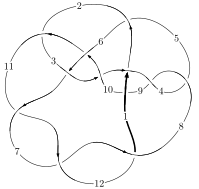
\includegraphics[width=112pt]{../../../GIT/diagram.site/Diagrams/png/2972_12n_0883.png}\\
\ \ \ A knot diagram\footnotemark}&
\allowdisplaybreaks
\textbf{Linearized knot diagam} \\
\cline{2-2}
 &
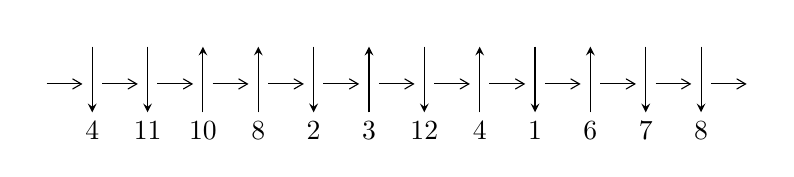
\begin{tikzpicture}[x=20pt, y=17pt]
	% nodes
	\node (C0) at (0, 0) {};
	\node (C1) at (1, 0) {};
	\node (C1U) at (1, +1) {};
	\node (C1D) at (1, -1) {4};

	\node (C2) at (2, 0) {};
	\node (C2U) at (2, +1) {};
	\node (C2D) at (2, -1) {11};

	\node (C3) at (3, 0) {};
	\node (C3U) at (3, +1) {};
	\node (C3D) at (3, -1) {10};

	\node (C4) at (4, 0) {};
	\node (C4U) at (4, +1) {};
	\node (C4D) at (4, -1) {8};

	\node (C5) at (5, 0) {};
	\node (C5U) at (5, +1) {};
	\node (C5D) at (5, -1) {2};

	\node (C6) at (6, 0) {};
	\node (C6U) at (6, +1) {};
	\node (C6D) at (6, -1) {3};

	\node (C7) at (7, 0) {};
	\node (C7U) at (7, +1) {};
	\node (C7D) at (7, -1) {12};

	\node (C8) at (8, 0) {};
	\node (C8U) at (8, +1) {};
	\node (C8D) at (8, -1) {4};

	\node (C9) at (9, 0) {};
	\node (C9U) at (9, +1) {};
	\node (C9D) at (9, -1) {1};

	\node (C10) at (10, 0) {};
	\node (C10U) at (10, +1) {};
	\node (C10D) at (10, -1) {6};

	\node (C11) at (11, 0) {};
	\node (C11U) at (11, +1) {};
	\node (C11D) at (11, -1) {7};

	\node (C12) at (12, 0) {};
	\node (C12U) at (12, +1) {};
	\node (C12D) at (12, -1) {8};
	\node (C13) at (13, 0) {};

	% arrows
	\draw[->,>={angle 60}]
	(C0) edge (C1) (C1) edge (C2) (C2) edge (C3) (C3) edge (C4) (C4) edge (C5) (C5) edge (C6) (C6) edge (C7) (C7) edge (C8) (C8) edge (C9) (C9) edge (C10) (C10) edge (C11) (C11) edge (C12) (C12) edge (C13) ;	\draw[->,>=stealth]
	(C1U) edge (C1D) (C2U) edge (C2D) (C3D) edge (C3U) (C4D) edge (C4U) (C5U) edge (C5D) (C6D) edge (C6U) (C7U) edge (C7D) (C8D) edge (C8U) (C9U) edge (C9D) (C10D) edge (C10U) (C11U) edge (C11D) (C12U) edge (C12D) ;
	\end{tikzpicture} \\
\hhline{~~} \\& 
\textbf{Solving Sequence} \\ \cline{2-2} 
 &
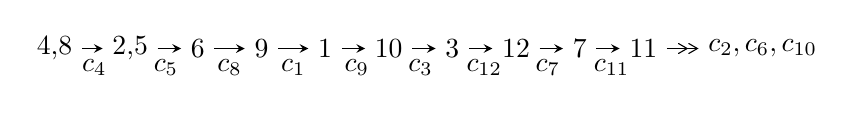
\begin{tikzpicture}[x=23pt, y=7pt]
	% node
	\node (A0) at (-1/8, 0) {4,8};
	\node (A1) at (17/16, 0) {2,5};
	\node (A2) at (17/8, 0) {6};
	\node (A3) at (25/8, 0) {9};
	\node (A4) at (33/8, 0) {1};
	\node (A5) at (41/8, 0) {10};
	\node (A6) at (49/8, 0) {3};
	\node (A7) at (57/8, 0) {12};
	\node (A8) at (65/8, 0) {7};
	\node (A9) at (73/8, 0) {11};
	\node (C1) at (1/2, -1) {$c_{4}$};
	\node (C2) at (13/8, -1) {$c_{5}$};
	\node (C3) at (21/8, -1) {$c_{8}$};
	\node (C4) at (29/8, -1) {$c_{1}$};
	\node (C5) at (37/8, -1) {$c_{9}$};
	\node (C6) at (45/8, -1) {$c_{3}$};
	\node (C7) at (53/8, -1) {$c_{12}$};
	\node (C8) at (61/8, -1) {$c_{7}$};
	\node (C9) at (69/8, -1) {$c_{11}$};
	\node (A10) at (11, 0) {$c_{2},c_{6},c_{10}$};

	% edge
	\draw[->,>=stealth]	
	(A0) edge (A1) (A1) edge (A2) (A2) edge (A3) (A3) edge (A4) (A4) edge (A5) (A5) edge (A6) (A6) edge (A7) (A7) edge (A8) (A8) edge (A9) ;
	\draw[->>,>={angle 60}]	
	(A9) edge (A10);
\end{tikzpicture} \\ 

\end{tabular} \\

\footnotetext{
The image of knot diagram is generated by the software ``\textbf{Draw programme}" developed by Andrew Bartholomew(\url{http://www.layer8.co.uk/maths/draw/index.htm\#Running-draw}), where we modified some parts for our purpose(\url{https://github.com/CATsTAILs/LinksPainter}).
}\phantom \\ \newline 
\centering \textbf{Ideals for irreducible components\footnotemark of $X_{\text{par}}$} 
 
\begin{align*}
I^u_{1}&=\langle 
1.59510\times10^{260} u^{68}-7.42718\times10^{260} u^{67}+\cdots+1.62945\times10^{263} b+1.10045\times10^{264},\\
\phantom{I^u_{1}}&\phantom{= \langle  }2.38672\times10^{264} u^{68}-1.77424\times10^{264} u^{67}+\cdots+2.65600\times10^{265} a+4.40019\times10^{267},\\
\phantom{I^u_{1}}&\phantom{= \langle  }u^{69}- u^{68}+\cdots+5598 u-326\rangle \\
I^u_{2}&=\langle 
4.71127\times10^{15} u^{19}-6.47791\times10^{15} u^{18}+\cdots+4.46458\times10^{16} b+2.86340\times10^{16},\\
\phantom{I^u_{2}}&\phantom{= \langle  }2.26761\times10^{16} u^{19}-5.05266\times10^{16} u^{18}+\cdots+8.92916\times10^{16} a-2.11962\times10^{17},\;u^{20}-2 u^{19}+\cdots-2 u+2\rangle \\
\\
\end{align*}
\raggedright * 2 irreducible components of $\dim_{\mathbb{C}}=0$, with total 89 representations.\\
\footnotetext{All coefficients of polynomials are rational numbers. But the coefficients are sometimes approximated in decimal forms when there is not enough margin.}
\newpage
\renewcommand{\arraystretch}{1}
\centering \section*{I. $I^u_{1}= \langle 1.60\times10^{260} u^{68}-7.43\times10^{260} u^{67}+\cdots+1.63\times10^{263} b+1.10\times10^{264},\;2.39\times10^{264} u^{68}-1.77\times10^{264} u^{67}+\cdots+2.66\times10^{265} a+4.40\times10^{267},\;u^{69}- u^{68}+\cdots+5598 u-326 \rangle$}
\flushleft \textbf{(i) Arc colorings}\\
\begin{tabular}{m{7pt} m{180pt} m{7pt} m{180pt} }
\flushright $a_{4}=$&$\begin{pmatrix}1\\0\end{pmatrix}$ \\
\flushright $a_{8}=$&$\begin{pmatrix}0\\u\end{pmatrix}$ \\
\flushright $a_{2}=$&$\begin{pmatrix}-0.0898616 u^{68}+0.0668011 u^{67}+\cdots+1857.03 u-165.670\\-0.000978922 u^{68}+0.00455810 u^{67}+\cdots+61.7443 u-6.75351\end{pmatrix}$ \\
\flushright $a_{5}=$&$\begin{pmatrix}1\\- u^2\end{pmatrix}$ \\
\flushright $a_{6}=$&$\begin{pmatrix}0.119212 u^{68}-0.0882484 u^{67}+\cdots-2414.13 u+212.151\\-0.0136947 u^{68}+0.00153908 u^{67}+\cdots+13.6473 u+5.88030\end{pmatrix}$ \\
\flushright $a_{9}=$&$\begin{pmatrix}u\\u\end{pmatrix}$ \\
\flushright $a_{1}=$&$\begin{pmatrix}-0.0908405 u^{68}+0.0713592 u^{67}+\cdots+1918.77 u-172.423\\-0.000978922 u^{68}+0.00455810 u^{67}+\cdots+61.7443 u-6.75351\end{pmatrix}$ \\
\flushright $a_{10}=$&$\begin{pmatrix}-0.0359205 u^{68}+0.0140602 u^{67}+\cdots+385.225 u-23.0840\\-0.0189792 u^{68}+0.0123122 u^{67}+\cdots+377.671 u-33.9102\end{pmatrix}$ \\
\flushright $a_{3}=$&$\begin{pmatrix}-0.0963752 u^{68}+0.0735527 u^{67}+\cdots+1908.00 u-163.170\\-0.00161754 u^{68}+0.00623717 u^{67}+\cdots+185.450 u-20.1627\end{pmatrix}$ \\
\flushright $a_{12}=$&$\begin{pmatrix}-0.0908405 u^{68}+0.0713592 u^{67}+\cdots+1918.77 u-172.423\\0.00621827 u^{68}+0.00190635 u^{67}+\cdots-17.6980 u-0.402606\end{pmatrix}$ \\
\flushright $a_{7}=$&$\begin{pmatrix}0.0373943 u^{68}-0.0234926 u^{67}+\cdots-647.218 u+50.3563\\-0.00842474 u^{68}-0.00858578 u^{67}+\cdots-196.363 u+22.7404\end{pmatrix}$ \\
\flushright $a_{11}=$&$\begin{pmatrix}-0.0936309 u^{68}+0.100845 u^{67}+\cdots+2668.46 u-251.034\\-0.00234625 u^{68}-0.00660391 u^{67}+\cdots-141.177 u+11.7322\end{pmatrix}$\\&\end{tabular}
\flushleft \textbf{(ii) Obstruction class $= -1$}\\~\\
\flushleft \textbf{(iii) Cusp Shapes $= 0.0737369 u^{68}-0.0552753 u^{67}+\cdots-1897.44 u+179.175$}\\~\\
\newpage\renewcommand{\arraystretch}{1}
\flushleft \textbf{(iv) u-Polynomials at the component}\newline \\
\begin{tabular}{m{50pt}|m{274pt}}
Crossings & \hspace{64pt}u-Polynomials at each crossing \\
\hline $$\begin{aligned}c_{1}\end{aligned}$$&$\begin{aligned}
&u^{69}+3 u^{68}+\cdots-7855 u-844
\end{aligned}$\\
\hline $$\begin{aligned}c_{2}\end{aligned}$$&$\begin{aligned}
&u^{69}+4 u^{68}+\cdots-447 u-94
\end{aligned}$\\
\hline $$\begin{aligned}c_{3}\end{aligned}$$&$\begin{aligned}
&u^{69}+22 u^{67}+\cdots+4528 u+2690
\end{aligned}$\\
\hline $$\begin{aligned}c_{4},c_{8}\end{aligned}$$&$\begin{aligned}
&u^{69}+u^{68}+\cdots+5598 u+326
\end{aligned}$\\
\hline $$\begin{aligned}c_{5}\end{aligned}$$&$\begin{aligned}
&u^{69}+2 u^{67}+\cdots-96 u-10
\end{aligned}$\\
\hline $$\begin{aligned}c_{6}\end{aligned}$$&$\begin{aligned}
&u^{69}-5 u^{68}+\cdots-1042 u-242
\end{aligned}$\\
\hline $$\begin{aligned}c_{7},c_{11},c_{12}\end{aligned}$$&$\begin{aligned}
&u^{69}- u^{68}+\cdots+8 u+2
\end{aligned}$\\
\hline $$\begin{aligned}c_{9}\end{aligned}$$&$\begin{aligned}
&u^{69}+37 u^{67}+\cdots-12439 u+1286
\end{aligned}$\\
\hline $$\begin{aligned}c_{10}\end{aligned}$$&$\begin{aligned}
&u^{69}+2 u^{68}+\cdots+u+2
\end{aligned}$\\
\hline
\end{tabular}\\~\\
\newpage\renewcommand{\arraystretch}{1}
\flushleft \textbf{(v) Riley Polynomials at the component}\newline \\
\begin{tabular}{m{50pt}|m{274pt}}
Crossings & \hspace{64pt}Riley Polynomials at each crossing \\
\hline $$\begin{aligned}c_{1}\end{aligned}$$&$\begin{aligned}
&y^{69}+61 y^{68}+\cdots-33395831 y-712336
\end{aligned}$\\
\hline $$\begin{aligned}c_{2}\end{aligned}$$&$\begin{aligned}
&y^{69}-10 y^{68}+\cdots+187213 y-8836
\end{aligned}$\\
\hline $$\begin{aligned}c_{3}\end{aligned}$$&$\begin{aligned}
&y^{69}+44 y^{68}+\cdots-160249076 y-7236100
\end{aligned}$\\
\hline $$\begin{aligned}c_{4},c_{8}\end{aligned}$$&$\begin{aligned}
&y^{69}-71 y^{68}+\cdots+10709628 y-106276
\end{aligned}$\\
\hline $$\begin{aligned}c_{5}\end{aligned}$$&$\begin{aligned}
&y^{69}+4 y^{68}+\cdots-111724 y-100
\end{aligned}$\\
\hline $$\begin{aligned}c_{6}\end{aligned}$$&$\begin{aligned}
&y^{69}+29 y^{68}+\cdots-1680780 y-58564
\end{aligned}$\\
\hline $$\begin{aligned}c_{7},c_{11},c_{12}\end{aligned}$$&$\begin{aligned}
&y^{69}-69 y^{68}+\cdots-1868 y-4
\end{aligned}$\\
\hline $$\begin{aligned}c_{9}\end{aligned}$$&$\begin{aligned}
&y^{69}+74 y^{68}+\cdots-48598167 y-1653796
\end{aligned}$\\
\hline $$\begin{aligned}c_{10}\end{aligned}$$&$\begin{aligned}
&y^{69}+70 y^{67}+\cdots-99 y-4
\end{aligned}$\\
\hline
\end{tabular}\\~\\
\newpage\flushleft \textbf{(vi) Complex Volumes and Cusp Shapes}
$$\begin{array}{c|c|c}  
\text{Solutions to }I^u_{1}& \I (\text{vol} + \sqrt{-1}CS) & \text{Cusp shape}\\
 \hline 
\begin{aligned}
u &= -0.937388 + 0.169929 I \\
a &= \phantom{-}0.043478 - 0.742272 I \\
b &= -1.43395 + 0.18421 I\end{aligned}
 & -7.84748 - 8.49945 I & \phantom{-0.000000 } 0 \\ \hline\begin{aligned}
u &= -0.937388 - 0.169929 I \\
a &= \phantom{-}0.043478 + 0.742272 I \\
b &= -1.43395 - 0.18421 I\end{aligned}
 & -7.84748 + 8.49945 I & \phantom{-0.000000 } 0 \\ \hline\begin{aligned}
u &= -0.900734 + 0.543791 I \\
a &= -0.880354 + 0.906296 I \\
b &= -0.10421 - 1.57726 I\end{aligned}
 & -0.86538 + 2.81593 I & \phantom{-0.000000 } 0 \\ \hline\begin{aligned}
u &= -0.900734 - 0.543791 I \\
a &= -0.880354 - 0.906296 I \\
b &= -0.10421 + 1.57726 I\end{aligned}
 & -0.86538 - 2.81593 I & \phantom{-0.000000 } 0 \\ \hline\begin{aligned}
u &= \phantom{-}0.901600 + 0.002839 I \\
a &= -0.299924 - 1.023530 I \\
b &= -1.241240 + 0.577767 I\end{aligned}
 & -6.61914 + 0.01529 I & \phantom{-0.000000 } 0 \\ \hline\begin{aligned}
u &= \phantom{-}0.901600 - 0.002839 I \\
a &= -0.299924 + 1.023530 I \\
b &= -1.241240 - 0.577767 I\end{aligned}
 & -6.61914 - 0.01529 I & \phantom{-0.000000 } 0 \\ \hline\begin{aligned}
u &= -1.098090 + 0.089462 I \\
a &= -0.231231 + 0.492442 I \\
b &= \phantom{-}1.47104 - 0.43938 I\end{aligned}
 & -6.40650 + 1.70687 I & \phantom{-0.000000 } 0 \\ \hline\begin{aligned}
u &= -1.098090 - 0.089462 I \\
a &= -0.231231 - 0.492442 I \\
b &= \phantom{-}1.47104 + 0.43938 I\end{aligned}
 & -6.40650 - 1.70687 I & \phantom{-0.000000 } 0 \\ \hline\begin{aligned}
u &= \phantom{-}0.891922\phantom{ +0.000000I} \\
a &= -1.33838\phantom{ +0.000000I} \\
b &= -0.319994\phantom{ +0.000000I}\end{aligned}
 & -3.90346\phantom{ +0.000000I} & \phantom{-0.000000 } 0 \\ \hline\begin{aligned}
u &= \phantom{-}1.084820 + 0.583325 I \\
a &= \phantom{-}0.429051 + 0.576072 I \\
b &= \phantom{-}0.30747 - 1.40594 I\end{aligned}
 & -1.38126 + 4.86406 I & \phantom{-0.000000 } 0\\
 \hline 
 \end{array}$$\newpage$$\begin{array}{c|c|c}  
\text{Solutions to }I^u_{1}& \I (\text{vol} + \sqrt{-1}CS) & \text{Cusp shape}\\
 \hline 
\begin{aligned}
u &= \phantom{-}1.084820 - 0.583325 I \\
a &= \phantom{-}0.429051 - 0.576072 I \\
b &= \phantom{-}0.30747 + 1.40594 I\end{aligned}
 & -1.38126 - 4.86406 I & \phantom{-0.000000 } 0 \\ \hline\begin{aligned}
u &= \phantom{-}0.122701 + 0.739942 I \\
a &= -0.892972 + 0.209852 I \\
b &= \phantom{-}0.443092 + 0.333001 I\end{aligned}
 & -1.26816 - 1.18876 I & -2.82487 + 5.99212 I \\ \hline\begin{aligned}
u &= \phantom{-}0.122701 - 0.739942 I \\
a &= -0.892972 - 0.209852 I \\
b &= \phantom{-}0.443092 - 0.333001 I\end{aligned}
 & -1.26816 + 1.18876 I & -2.82487 - 5.99212 I \\ \hline\begin{aligned}
u &= -0.521137 + 0.477077 I \\
a &= \phantom{-}1.87070 + 2.12252 I \\
b &= -0.053829 - 0.734075 I\end{aligned}
 & -9.29987 + 6.46112 I & -3.09471 - 4.46072 I \\ \hline\begin{aligned}
u &= -0.521137 - 0.477077 I \\
a &= \phantom{-}1.87070 - 2.12252 I \\
b &= -0.053829 + 0.734075 I\end{aligned}
 & -9.29987 - 6.46112 I & -3.09471 + 4.46072 I \\ \hline\begin{aligned}
u &= \phantom{-}0.616847 + 0.305370 I \\
a &= \phantom{-}0.386621 - 0.542148 I \\
b &= \phantom{-}1.270370 - 0.229148 I\end{aligned}
 & -5.74954 + 1.06735 I & -12.5664 - 6.4993 I \\ \hline\begin{aligned}
u &= \phantom{-}0.616847 - 0.305370 I \\
a &= \phantom{-}0.386621 + 0.542148 I \\
b &= \phantom{-}1.270370 + 0.229148 I\end{aligned}
 & -5.74954 - 1.06735 I & -12.5664 + 6.4993 I \\ \hline\begin{aligned}
u &= \phantom{-}1.315000 + 0.102944 I \\
a &= -0.278028 + 1.229770 I \\
b &= \phantom{-}0.39050 - 1.53129 I\end{aligned}
 & \phantom{-}2.43759 + 4.36021 I & \phantom{-0.000000 } 0 \\ \hline\begin{aligned}
u &= \phantom{-}1.315000 - 0.102944 I \\
a &= -0.278028 - 1.229770 I \\
b &= \phantom{-}0.39050 + 1.53129 I\end{aligned}
 & \phantom{-}2.43759 - 4.36021 I & \phantom{-0.000000 } 0 \\ \hline\begin{aligned}
u &= \phantom{-}0.294280 + 0.543366 I \\
a &= \phantom{-}1.01357 - 1.53056 I \\
b &= \phantom{-}0.314876 - 0.875991 I\end{aligned}
 & -8.76029 + 1.21269 I & -5.57587 - 5.50908 I\\
 \hline 
 \end{array}$$\newpage$$\begin{array}{c|c|c}  
\text{Solutions to }I^u_{1}& \I (\text{vol} + \sqrt{-1}CS) & \text{Cusp shape}\\
 \hline 
\begin{aligned}
u &= \phantom{-}0.294280 - 0.543366 I \\
a &= \phantom{-}1.01357 + 1.53056 I \\
b &= \phantom{-}0.314876 + 0.875991 I\end{aligned}
 & -8.76029 - 1.21269 I & -5.57587 + 5.50908 I \\ \hline\begin{aligned}
u &= -0.456789 + 0.317551 I \\
a &= -0.559476 + 0.192992 I \\
b &= -0.115002 + 0.434041 I\end{aligned}
 & \phantom{-}0.98160 - 1.05730 I & \phantom{-}2.65855 + 2.72887 I \\ \hline\begin{aligned}
u &= -0.456789 - 0.317551 I \\
a &= -0.559476 - 0.192992 I \\
b &= -0.115002 - 0.434041 I\end{aligned}
 & \phantom{-}0.98160 + 1.05730 I & \phantom{-}2.65855 - 2.72887 I \\ \hline\begin{aligned}
u &= \phantom{-}0.27792 + 1.43387 I \\
a &= \phantom{-}0.184504 - 0.104863 I \\
b &= \phantom{-}0.169303 - 0.837058 I\end{aligned}
 & -8.67747 + 0.45721 I & \phantom{-0.000000 } 0 \\ \hline\begin{aligned}
u &= \phantom{-}0.27792 - 1.43387 I \\
a &= \phantom{-}0.184504 + 0.104863 I \\
b &= \phantom{-}0.169303 + 0.837058 I\end{aligned}
 & -8.67747 - 0.45721 I & \phantom{-0.000000 } 0 \\ \hline\begin{aligned}
u &= -0.14990 + 1.48458 I \\
a &= \phantom{-}0.315672 + 0.178950 I \\
b &= \phantom{-}0.085797 - 0.238221 I\end{aligned}
 & -3.99806 - 3.95956 I & \phantom{-0.000000 } 0 \\ \hline\begin{aligned}
u &= -0.14990 - 1.48458 I \\
a &= \phantom{-}0.315672 - 0.178950 I \\
b &= \phantom{-}0.085797 + 0.238221 I\end{aligned}
 & -3.99806 + 3.95956 I & \phantom{-0.000000 } 0 \\ \hline\begin{aligned}
u &= \phantom{-}0.349929 + 0.366099 I \\
a &= -1.39394 + 0.39447 I \\
b &= \phantom{-}0.190178 + 0.220324 I\end{aligned}
 & -1.21862 - 0.72825 I & -4.93688 + 0.50068 I \\ \hline\begin{aligned}
u &= \phantom{-}0.349929 - 0.366099 I \\
a &= -1.39394 - 0.39447 I \\
b &= \phantom{-}0.190178 - 0.220324 I\end{aligned}
 & -1.21862 + 0.72825 I & -4.93688 - 0.50068 I \\ \hline\begin{aligned}
u &= \phantom{-}0.402832 + 0.287203 I \\
a &= -0.958411 - 0.330421 I \\
b &= \phantom{-}1.015600 + 0.448453 I\end{aligned}
 & -1.86231 - 1.13742 I & \phantom{-}2.46556 - 4.13256 I\\
 \hline 
 \end{array}$$\newpage$$\begin{array}{c|c|c}  
\text{Solutions to }I^u_{1}& \I (\text{vol} + \sqrt{-1}CS) & \text{Cusp shape}\\
 \hline 
\begin{aligned}
u &= \phantom{-}0.402832 - 0.287203 I \\
a &= -0.958411 + 0.330421 I \\
b &= \phantom{-}1.015600 - 0.448453 I\end{aligned}
 & -1.86231 + 1.13742 I & \phantom{-}2.46556 + 4.13256 I \\ \hline\begin{aligned}
u &= -1.37941 + 0.63523 I \\
a &= \phantom{-}0.495306 - 1.088720 I \\
b &= \phantom{-}0.31114 + 1.68003 I\end{aligned}
 & \phantom{-}1.20843 - 8.06995 I & \phantom{-0.000000 } 0 \\ \hline\begin{aligned}
u &= -1.37941 - 0.63523 I \\
a &= \phantom{-}0.495306 + 1.088720 I \\
b &= \phantom{-}0.31114 - 1.68003 I\end{aligned}
 & \phantom{-}1.20843 + 8.06995 I & \phantom{-0.000000 } 0 \\ \hline\begin{aligned}
u &= -1.54862 + 0.18920 I \\
a &= \phantom{-}0.531241 - 0.765048 I \\
b &= -0.02146 + 1.56991 I\end{aligned}
 & \phantom{-}2.62752 + 3.54439 I & \phantom{-0.000000 } 0 \\ \hline\begin{aligned}
u &= -1.54862 - 0.18920 I \\
a &= \phantom{-}0.531241 + 0.765048 I \\
b &= -0.02146 - 1.56991 I\end{aligned}
 & \phantom{-}2.62752 - 3.54439 I & \phantom{-0.000000 } 0 \\ \hline\begin{aligned}
u &= \phantom{-}0.426848 + 0.055916 I \\
a &= \phantom{-}1.94065 - 0.16496 I \\
b &= \phantom{-}0.013936 + 0.901571 I\end{aligned}
 & -1.20775 - 4.21129 I & -4.14353 + 6.76110 I \\ \hline\begin{aligned}
u &= \phantom{-}0.426848 - 0.055916 I \\
a &= \phantom{-}1.94065 + 0.16496 I \\
b &= \phantom{-}0.013936 - 0.901571 I\end{aligned}
 & -1.20775 + 4.21129 I & -4.14353 - 6.76110 I \\ \hline\begin{aligned}
u &= -1.58578 + 0.06116 I \\
a &= \phantom{-}0.216735 + 0.784957 I \\
b &= -0.28573 - 1.56489 I\end{aligned}
 & \phantom{-}2.33854 - 1.02618 I & \phantom{-0.000000 } 0 \\ \hline\begin{aligned}
u &= -1.58578 - 0.06116 I \\
a &= \phantom{-}0.216735 - 0.784957 I \\
b &= -0.28573 + 1.56489 I\end{aligned}
 & \phantom{-}2.33854 + 1.02618 I & \phantom{-0.000000 } 0 \\ \hline\begin{aligned}
u &= -0.316446 + 0.256770 I \\
a &= -3.53853 - 1.87963 I \\
b &= \phantom{-}0.422485 - 0.553073 I\end{aligned}
 & -9.07448 + 1.51500 I & \phantom{-}2.38611 + 3.76927 I\\
 \hline 
 \end{array}$$\newpage$$\begin{array}{c|c|c}  
\text{Solutions to }I^u_{1}& \I (\text{vol} + \sqrt{-1}CS) & \text{Cusp shape}\\
 \hline 
\begin{aligned}
u &= -0.316446 - 0.256770 I \\
a &= -3.53853 + 1.87963 I \\
b &= \phantom{-}0.422485 + 0.553073 I\end{aligned}
 & -9.07448 - 1.51500 I & \phantom{-}2.38611 - 3.76927 I \\ \hline\begin{aligned}
u &= -1.53034 + 0.45332 I \\
a &= \phantom{-}0.051803 - 1.168240 I \\
b &= \phantom{-}0.76970 + 1.51354 I\end{aligned}
 & -2.82820 - 6.39077 I & \phantom{-0.000000 } 0 \\ \hline\begin{aligned}
u &= -1.53034 - 0.45332 I \\
a &= \phantom{-}0.051803 + 1.168240 I \\
b &= \phantom{-}0.76970 - 1.51354 I\end{aligned}
 & -2.82820 + 6.39077 I & \phantom{-0.000000 } 0 \\ \hline\begin{aligned}
u &= \phantom{-}1.59807 + 0.28399 I \\
a &= \phantom{-}0.144623 + 1.087600 I \\
b &= \phantom{-}0.00268 - 1.61595 I\end{aligned}
 & \phantom{-}7.27344 + 4.05568 I & \phantom{-0.000000 } 0 \\ \hline\begin{aligned}
u &= \phantom{-}1.59807 - 0.28399 I \\
a &= \phantom{-}0.144623 - 1.087600 I \\
b &= \phantom{-}0.00268 + 1.61595 I\end{aligned}
 & \phantom{-}7.27344 - 4.05568 I & \phantom{-0.000000 } 0 \\ \hline\begin{aligned}
u &= \phantom{-}1.59921 + 0.31569 I \\
a &= -0.589281 - 0.847626 I \\
b &= -0.121264 + 1.185740 I\end{aligned}
 & \phantom{-}0.519660 + 0.341918 I & \phantom{-0.000000 } 0 \\ \hline\begin{aligned}
u &= \phantom{-}1.59921 - 0.31569 I \\
a &= -0.589281 + 0.847626 I \\
b &= -0.121264 - 1.185740 I\end{aligned}
 & \phantom{-}0.519660 - 0.341918 I & \phantom{-0.000000 } 0 \\ \hline\begin{aligned}
u &= -1.66807 + 0.10006 I \\
a &= -0.148154 + 0.990473 I \\
b &= -0.35286 - 1.39288 I\end{aligned}
 & \phantom{-}5.90864 - 0.86319 I & \phantom{-0.000000 } 0 \\ \hline\begin{aligned}
u &= -1.66807 - 0.10006 I \\
a &= -0.148154 - 0.990473 I \\
b &= -0.35286 + 1.39288 I\end{aligned}
 & \phantom{-}5.90864 + 0.86319 I & \phantom{-0.000000 } 0 \\ \hline\begin{aligned}
u &= \phantom{-}1.42486 + 0.88427 I \\
a &= -0.543349 - 0.812666 I \\
b &= -0.073113 + 1.322830 I\end{aligned}
 & \phantom{-}0.34448 + 1.46095 I & \phantom{-0.000000 } 0\\
 \hline 
 \end{array}$$\newpage$$\begin{array}{c|c|c}  
\text{Solutions to }I^u_{1}& \I (\text{vol} + \sqrt{-1}CS) & \text{Cusp shape}\\
 \hline 
\begin{aligned}
u &= \phantom{-}1.42486 - 0.88427 I \\
a &= -0.543349 + 0.812666 I \\
b &= -0.073113 - 1.322830 I\end{aligned}
 & \phantom{-}0.34448 - 1.46095 I & \phantom{-0.000000 } 0 \\ \hline\begin{aligned}
u &= -1.65530 + 0.35198 I \\
a &= -0.228611 - 1.013180 I \\
b &= \phantom{-}0.14810 + 1.42442 I\end{aligned}
 & \phantom{-}4.34530 - 3.39833 I & \phantom{-0.000000 } 0 \\ \hline\begin{aligned}
u &= -1.65530 - 0.35198 I \\
a &= -0.228611 + 1.013180 I \\
b &= \phantom{-}0.14810 - 1.42442 I\end{aligned}
 & \phantom{-}4.34530 + 3.39833 I & \phantom{-0.000000 } 0 \\ \hline\begin{aligned}
u &= \phantom{-}1.67896 + 0.56416 I \\
a &= -0.062341 - 0.915295 I \\
b &= -0.69881 + 1.44153 I\end{aligned}
 & -3.54897 + 7.24525 I & \phantom{-0.000000 } 0 \\ \hline\begin{aligned}
u &= \phantom{-}1.67896 - 0.56416 I \\
a &= -0.062341 + 0.915295 I \\
b &= -0.69881 - 1.44153 I\end{aligned}
 & -3.54897 - 7.24525 I & \phantom{-0.000000 } 0 \\ \hline\begin{aligned}
u &= \phantom{-}1.74673 + 0.30476 I \\
a &= \phantom{-}0.194566 - 0.972442 I \\
b &= -0.38911 + 1.61323 I\end{aligned}
 & \phantom{-}3.46954 + 10.71400 I & \phantom{-0.000000 } 0 \\ \hline\begin{aligned}
u &= \phantom{-}1.74673 - 0.30476 I \\
a &= \phantom{-}0.194566 + 0.972442 I \\
b &= -0.38911 - 1.61323 I\end{aligned}
 & \phantom{-}3.46954 - 10.71400 I & \phantom{-0.000000 } 0 \\ \hline\begin{aligned}
u &= \phantom{-}1.48603 + 0.98544 I \\
a &= \phantom{-}0.129346 + 1.000480 I \\
b &= \phantom{-}0.39902 - 1.52526 I\end{aligned}
 & \phantom{-}0.25276 + 6.84890 I & \phantom{-0.000000 } 0 \\ \hline\begin{aligned}
u &= \phantom{-}1.48603 - 0.98544 I \\
a &= \phantom{-}0.129346 - 1.000480 I \\
b &= \phantom{-}0.39902 + 1.52526 I\end{aligned}
 & \phantom{-}0.25276 - 6.84890 I & \phantom{-0.000000 } 0 \\ \hline\begin{aligned}
u &= -1.79984 + 0.31515 I \\
a &= -0.209297 + 1.015280 I \\
b &= \phantom{-}0.213560 - 1.208730 I\end{aligned}
 & \phantom{-}4.92575 + 0.66345 I & \phantom{-0.000000 } 0\\
 \hline 
 \end{array}$$\newpage$$\begin{array}{c|c|c}  
\text{Solutions to }I^u_{1}& \I (\text{vol} + \sqrt{-1}CS) & \text{Cusp shape}\\
 \hline 
\begin{aligned}
u &= -1.79984 - 0.31515 I \\
a &= -0.209297 - 1.015280 I \\
b &= \phantom{-}0.213560 + 1.208730 I\end{aligned}
 & \phantom{-}4.92575 - 0.66345 I & \phantom{-0.000000 } 0 \\ \hline\begin{aligned}
u &= \phantom{-}0.166218 + 0.017157 I \\
a &= \phantom{-}0.82946 + 4.69831 I \\
b &= -1.264600 + 0.167920 I\end{aligned}
 & -2.81269 + 4.67156 I & -3.12185 - 6.15405 I \\ \hline\begin{aligned}
u &= \phantom{-}0.166218 - 0.017157 I \\
a &= \phantom{-}0.82946 - 4.69831 I \\
b &= -1.264600 - 0.167920 I\end{aligned}
 & -2.81269 - 4.67156 I & -3.12185 + 6.15405 I \\ \hline\begin{aligned}
u &= -1.74104 + 0.69909 I \\
a &= -0.054215 + 1.043500 I \\
b &= -0.64425 - 1.54738 I\end{aligned}
 & -3.2595 - 15.9571 I & \phantom{-0.000000 } 0 \\ \hline\begin{aligned}
u &= -1.74104 - 0.69909 I \\
a &= -0.054215 - 1.043500 I \\
b &= -0.64425 + 1.54738 I\end{aligned}
 & -3.2595 + 15.9571 I & \phantom{-0.000000 } 0 \\ \hline\begin{aligned}
u &= -0.26113 + 1.90968 I \\
a &= \phantom{-}0.237425 - 0.276892 I \\
b &= -0.036362 + 0.960242 I\end{aligned}
 & -8.52014 + 6.77449 I & \phantom{-0.000000 } 0 \\ \hline\begin{aligned}
u &= -0.26113 - 1.90968 I \\
a &= \phantom{-}0.237425 + 0.276892 I \\
b &= -0.036362 - 0.960242 I\end{aligned}
 & -8.52014 - 6.77449 I & \phantom{-0.000000 } 0 \\ \hline\begin{aligned}
u &= \phantom{-}2.11120 + 0.09785 I \\
a &= \phantom{-}0.086951 + 0.988989 I \\
b &= \phantom{-}0.556942 - 1.075320 I\end{aligned}
 & \phantom{-}0.48418 + 2.25326 I & \phantom{-0.000000 } 0 \\ \hline\begin{aligned}
u &= \phantom{-}2.11120 - 0.09785 I \\
a &= \phantom{-}0.086951 - 0.988989 I \\
b &= \phantom{-}0.556942 + 1.075320 I\end{aligned}
 & \phantom{-}0.48418 - 2.25326 I & \phantom{-0.000000 } 0\\
 \hline 
 \end{array}$$\newpage\newpage\renewcommand{\arraystretch}{1}
\centering \section*{II. $I^u_{2}= \langle 4.71\times10^{15} u^{19}-6.48\times10^{15} u^{18}+\cdots+4.46\times10^{16} b+2.86\times10^{16},\;2.27\times10^{16} u^{19}-5.05\times10^{16} u^{18}+\cdots+8.93\times10^{16} a-2.12\times10^{17},\;u^{20}-2 u^{19}+\cdots-2 u+2 \rangle$}
\flushleft \textbf{(i) Arc colorings}\\
\begin{tabular}{m{7pt} m{180pt} m{7pt} m{180pt} }
\flushright $a_{4}=$&$\begin{pmatrix}1\\0\end{pmatrix}$ \\
\flushright $a_{8}=$&$\begin{pmatrix}0\\u\end{pmatrix}$ \\
\flushright $a_{2}=$&$\begin{pmatrix}-0.253955 u^{19}+0.565861 u^{18}+\cdots-4.57373 u+2.37382\\-0.105525 u^{19}+0.145096 u^{18}+\cdots-0.367388 u-0.641359\end{pmatrix}$ \\
\flushright $a_{5}=$&$\begin{pmatrix}1\\- u^2\end{pmatrix}$ \\
\flushright $a_{6}=$&$\begin{pmatrix}0.0104055 u^{19}-0.126171 u^{18}+\cdots+3.06894 u-0.296781\\0.0899192 u^{19}-0.130317 u^{18}+\cdots-0.138878 u+0.437370\end{pmatrix}$ \\
\flushright $a_{9}=$&$\begin{pmatrix}u\\u\end{pmatrix}$ \\
\flushright $a_{1}=$&$\begin{pmatrix}-0.359480 u^{19}+0.710956 u^{18}+\cdots-4.94112 u+1.73246\\-0.105525 u^{19}+0.145096 u^{18}+\cdots-0.367388 u-0.641359\end{pmatrix}$ \\
\flushright $a_{10}=$&$\begin{pmatrix}0.903364 u^{19}-1.70724 u^{18}+\cdots+6.10414 u-3.55956\\0.179321 u^{19}-0.253116 u^{18}+\cdots+3.73612 u+0.00874632\end{pmatrix}$ \\
\flushright $a_{3}=$&$\begin{pmatrix}0.315050 u^{19}-1.00867 u^{18}+\cdots-5.55543 u-6.78367\\0.355127 u^{19}-0.608260 u^{18}+\cdots+3.13098 u-1.15233\end{pmatrix}$ \\
\flushright $a_{12}=$&$\begin{pmatrix}-0.359480 u^{19}+0.710956 u^{18}+\cdots-4.94112 u+1.73246\\-0.206683 u^{19}+0.300685 u^{18}+\cdots-1.07034 u-0.657368\end{pmatrix}$ \\
\flushright $a_{7}=$&$\begin{pmatrix}-0.967208 u^{19}+1.77827 u^{18}+\cdots-7.37065 u+3.15992\\-0.0747343 u^{19}+0.110510 u^{18}+\cdots-2.88862 u-0.711932\end{pmatrix}$ \\
\flushright $a_{11}=$&$\begin{pmatrix}0.678448 u^{19}-1.42392 u^{18}+\cdots+7.26152 u-2.34715\\0.0557314 u^{19}-0.0278410 u^{18}+\cdots+3.34451 u+0.244000\end{pmatrix}$\\&\end{tabular}
\flushleft \textbf{(ii) Obstruction class $= 1$}\\~\\
\flushleft \textbf{(iii) Cusp Shapes $= \frac{21125193779764826}{44645823690514751} u^{19}-\frac{46994070852762617}{44645823690514751} u^{18}+\cdots+\frac{128450800382224996}{44645823690514751} u-\frac{896563895668882454}{44645823690514751}$}\\~\\
\newpage\renewcommand{\arraystretch}{1}
\flushleft \textbf{(iv) u-Polynomials at the component}\newline \\
\begin{tabular}{m{50pt}|m{274pt}}
Crossings & \hspace{64pt}u-Polynomials at each crossing \\
\hline $$\begin{aligned}c_{1}\end{aligned}$$&$\begin{aligned}
&u^{20}-4 u^{19}+\cdots+3 u+1
\end{aligned}$\\
\hline $$\begin{aligned}c_{2}\end{aligned}$$&$\begin{aligned}
&u^{20}-3 u^{19}+\cdots-5 u+1
\end{aligned}$\\
\hline $$\begin{aligned}c_{3}\end{aligned}$$&$\begin{aligned}
&u^{20}- u^{19}+\cdots-5 u+4
\end{aligned}$\\
\hline $$\begin{aligned}c_{4}\end{aligned}$$&$\begin{aligned}
&u^{20}-2 u^{19}+\cdots-2 u+2
\end{aligned}$\\
\hline $$\begin{aligned}c_{5}\end{aligned}$$&$\begin{aligned}
&u^{20}-3 u^{19}+\cdots-45 u+26
\end{aligned}$\\
\hline $$\begin{aligned}c_{6}\end{aligned}$$&$\begin{aligned}
&u^{20}+7 u^{18}+\cdots-2 u+2
\end{aligned}$\\
\hline $$\begin{aligned}c_{7}\end{aligned}$$&$\begin{aligned}
&u^{20}-12 u^{18}+\cdots-5 u+2
\end{aligned}$\\
\hline $$\begin{aligned}c_{8}\end{aligned}$$&$\begin{aligned}
&u^{20}+2 u^{19}+\cdots+2 u+2
\end{aligned}$\\
\hline $$\begin{aligned}c_{9}\end{aligned}$$&$\begin{aligned}
&u^{20}+u^{19}+\cdots+14 u+7
\end{aligned}$\\
\hline $$\begin{aligned}c_{10}\end{aligned}$$&$\begin{aligned}
&u^{20}- u^{19}+\cdots+u+1
\end{aligned}$\\
\hline $$\begin{aligned}c_{11},c_{12}\end{aligned}$$&$\begin{aligned}
&u^{20}-12 u^{18}+\cdots+5 u+2
\end{aligned}$\\
\hline
\end{tabular}\\~\\
\newpage\renewcommand{\arraystretch}{1}
\flushleft \textbf{(v) Riley Polynomials at the component}\newline \\
\begin{tabular}{m{50pt}|m{274pt}}
Crossings & \hspace{64pt}Riley Polynomials at each crossing \\
\hline $$\begin{aligned}c_{1}\end{aligned}$$&$\begin{aligned}
&y^{20}+10 y^{19}+\cdots-11 y+1
\end{aligned}$\\
\hline $$\begin{aligned}c_{2}\end{aligned}$$&$\begin{aligned}
&y^{20}- y^{19}+\cdots-5 y+1
\end{aligned}$\\
\hline $$\begin{aligned}c_{3}\end{aligned}$$&$\begin{aligned}
&y^{20}+17 y^{19}+\cdots+215 y+16
\end{aligned}$\\
\hline $$\begin{aligned}c_{4},c_{8}\end{aligned}$$&$\begin{aligned}
&y^{20}-14 y^{19}+\cdots+24 y+4
\end{aligned}$\\
\hline $$\begin{aligned}c_{5}\end{aligned}$$&$\begin{aligned}
&y^{20}+13 y^{19}+\cdots-10865 y+676
\end{aligned}$\\
\hline $$\begin{aligned}c_{6}\end{aligned}$$&$\begin{aligned}
&y^{20}+14 y^{19}+\cdots+32 y+4
\end{aligned}$\\
\hline $$\begin{aligned}c_{7},c_{11},c_{12}\end{aligned}$$&$\begin{aligned}
&y^{20}-24 y^{19}+\cdots-41 y+4
\end{aligned}$\\
\hline $$\begin{aligned}c_{9}\end{aligned}$$&$\begin{aligned}
&y^{20}+11 y^{19}+\cdots-378 y+49
\end{aligned}$\\
\hline $$\begin{aligned}c_{10}\end{aligned}$$&$\begin{aligned}
&y^{20}-3 y^{19}+\cdots+11 y+1
\end{aligned}$\\
\hline
\end{tabular}\\~\\
\newpage\flushleft \textbf{(vi) Complex Volumes and Cusp Shapes}
$$\begin{array}{c|c|c}  
\text{Solutions to }I^u_{2}& \I (\text{vol} + \sqrt{-1}CS) & \text{Cusp shape}\\
 \hline 
\begin{aligned}
u &= \phantom{-}0.445341 + 1.006900 I \\
a &= \phantom{-}0.378996 - 0.609489 I \\
b &= \phantom{-}0.475822 - 0.653916 I\end{aligned}
 & -9.54640 + 0.43274 I & -14.2472 + 0.4571 I \\ \hline\begin{aligned}
u &= \phantom{-}0.445341 - 1.006900 I \\
a &= \phantom{-}0.378996 + 0.609489 I \\
b &= \phantom{-}0.475822 + 0.653916 I\end{aligned}
 & -9.54640 - 0.43274 I & -14.2472 - 0.4571 I \\ \hline\begin{aligned}
u &= -0.305160 + 1.095290 I \\
a &= \phantom{-}0.017343 + 1.275150 I \\
b &= \phantom{-}0.472191 - 0.019528 I\end{aligned}
 & -10.53160 + 6.61475 I & -10.62909 - 4.57987 I \\ \hline\begin{aligned}
u &= -0.305160 - 1.095290 I \\
a &= \phantom{-}0.017343 - 1.275150 I \\
b &= \phantom{-}0.472191 + 0.019528 I\end{aligned}
 & -10.53160 - 6.61475 I & -10.62909 + 4.57987 I \\ \hline\begin{aligned}
u &= \phantom{-}0.819504 + 0.038714 I \\
a &= -0.461140 + 0.552148 I \\
b &= -1.156310 - 0.340346 I\end{aligned}
 & -5.16397 - 0.27439 I & -4.64612 + 0.00082 I \\ \hline\begin{aligned}
u &= \phantom{-}0.819504 - 0.038714 I \\
a &= -0.461140 - 0.552148 I \\
b &= -1.156310 + 0.340346 I\end{aligned}
 & -5.16397 + 0.27439 I & -4.64612 - 0.00082 I \\ \hline\begin{aligned}
u &= \phantom{-}0.054278 + 1.230410 I \\
a &= -0.163473 - 0.310256 I \\
b &= \phantom{-}0.599474 + 0.188835 I\end{aligned}
 & -4.48083 - 4.26522 I & -11.29736 + 6.83205 I \\ \hline\begin{aligned}
u &= \phantom{-}0.054278 - 1.230410 I \\
a &= -0.163473 + 0.310256 I \\
b &= \phantom{-}0.599474 - 0.188835 I\end{aligned}
 & -4.48083 + 4.26522 I & -11.29736 - 6.83205 I \\ \hline\begin{aligned}
u &= -1.396840 + 0.098244 I \\
a &= \phantom{-}0.477139 - 0.906250 I \\
b &= -0.11675 + 1.53608 I\end{aligned}
 & \phantom{-}2.63581 + 2.60541 I & -3.56183 - 0.71884 I \\ \hline\begin{aligned}
u &= -1.396840 - 0.098244 I \\
a &= \phantom{-}0.477139 + 0.906250 I \\
b &= -0.11675 - 1.53608 I\end{aligned}
 & \phantom{-}2.63581 - 2.60541 I & -3.56183 + 0.71884 I\\
 \hline 
 \end{array}$$\newpage$$\begin{array}{c|c|c}  
\text{Solutions to }I^u_{2}& \I (\text{vol} + \sqrt{-1}CS) & \text{Cusp shape}\\
 \hline 
\begin{aligned}
u &= \phantom{-}1.33652 + 0.71442 I \\
a &= -0.185580 - 1.012890 I \\
b &= -0.48691 + 1.58830 I\end{aligned}
 & -0.48906 + 6.44073 I & -7.25375 - 5.52907 I \\ \hline\begin{aligned}
u &= \phantom{-}1.33652 - 0.71442 I \\
a &= -0.185580 + 1.012890 I \\
b &= -0.48691 - 1.58830 I\end{aligned}
 & -0.48906 - 6.44073 I & -7.25375 + 5.52907 I \\ \hline\begin{aligned}
u &= -0.291685 + 0.269932 I \\
a &= \phantom{-}1.83960 + 0.09965 I \\
b &= -0.920486 + 0.439782 I\end{aligned}
 & -2.17821 + 1.32113 I & -17.8526 - 7.1209 I \\ \hline\begin{aligned}
u &= -0.291685 - 0.269932 I \\
a &= \phantom{-}1.83960 - 0.09965 I \\
b &= -0.920486 - 0.439782 I\end{aligned}
 & -2.17821 - 1.32113 I & -17.8526 + 7.1209 I \\ \hline\begin{aligned}
u &= \phantom{-}0.164640 + 0.335831 I \\
a &= \phantom{-}2.58852 - 3.21941 I \\
b &= -0.684610 - 0.572192 I\end{aligned}
 & -9.34616 - 1.63192 I & -23.0792 + 7.1433 I \\ \hline\begin{aligned}
u &= \phantom{-}0.164640 - 0.335831 I \\
a &= \phantom{-}2.58852 + 3.21941 I \\
b &= -0.684610 + 0.572192 I\end{aligned}
 & -9.34616 + 1.63192 I & -23.0792 - 7.1433 I \\ \hline\begin{aligned}
u &= -1.76638 + 0.00494 I \\
a &= \phantom{-}0.060210 - 0.998278 I \\
b &= -0.323533 + 1.236200 I\end{aligned}
 & \phantom{-}4.58999 + 1.40746 I & -3.39132 - 5.03852 I \\ \hline\begin{aligned}
u &= -1.76638 - 0.00494 I \\
a &= \phantom{-}0.060210 + 0.998278 I \\
b &= -0.323533 - 1.236200 I\end{aligned}
 & \phantom{-}4.58999 - 1.40746 I & -3.39132 + 5.03852 I \\ \hline\begin{aligned}
u &= \phantom{-}1.93978 + 0.51365 I \\
a &= \phantom{-}0.448387 + 0.904270 I \\
b &= \phantom{-}0.141119 - 1.151680 I\end{aligned}
 & \phantom{-}1.61171 + 0.65918 I & \phantom{-}1.95852 + 0.33886 I \\ \hline\begin{aligned}
u &= \phantom{-}1.93978 - 0.51365 I \\
a &= \phantom{-}0.448387 - 0.904270 I \\
b &= \phantom{-}0.141119 + 1.151680 I\end{aligned}
 & \phantom{-}1.61171 - 0.65918 I & \phantom{-}1.95852 - 0.33886 I\\
 \hline 
 \end{array}$$\newpage
\newpage\renewcommand{\arraystretch}{1}
\centering \section*{ III. u-Polynomials}
\begin{tabular}{m{50pt}|m{274pt}}
Crossings & \hspace{64pt}u-Polynomials at each crossing \\
\hline $$\begin{aligned}c_{1}\end{aligned}$$&$\begin{aligned}
&(u^{20}-4 u^{19}+\cdots+3 u+1)(u^{69}+3 u^{68}+\cdots-7855 u-844)
\end{aligned}$\\
\hline $$\begin{aligned}c_{2}\end{aligned}$$&$\begin{aligned}
&(u^{20}-3 u^{19}+\cdots-5 u+1)(u^{69}+4 u^{68}+\cdots-447 u-94)
\end{aligned}$\\
\hline $$\begin{aligned}c_{3}\end{aligned}$$&$\begin{aligned}
&(u^{20}- u^{19}+\cdots-5 u+4)(u^{69}+22 u^{67}+\cdots+4528 u+2690)
\end{aligned}$\\
\hline $$\begin{aligned}c_{4}\end{aligned}$$&$\begin{aligned}
&(u^{20}-2 u^{19}+\cdots-2 u+2)(u^{69}+u^{68}+\cdots+5598 u+326)
\end{aligned}$\\
\hline $$\begin{aligned}c_{5}\end{aligned}$$&$\begin{aligned}
&(u^{20}-3 u^{19}+\cdots-45 u+26)(u^{69}+2 u^{67}+\cdots-96 u-10)
\end{aligned}$\\
\hline $$\begin{aligned}c_{6}\end{aligned}$$&$\begin{aligned}
&(u^{20}+7 u^{18}+\cdots-2 u+2)(u^{69}-5 u^{68}+\cdots-1042 u-242)
\end{aligned}$\\
\hline $$\begin{aligned}c_{7}\end{aligned}$$&$\begin{aligned}
&(u^{20}-12 u^{18}+\cdots-5 u+2)(u^{69}- u^{68}+\cdots+8 u+2)
\end{aligned}$\\
\hline $$\begin{aligned}c_{8}\end{aligned}$$&$\begin{aligned}
&(u^{20}+2 u^{19}+\cdots+2 u+2)(u^{69}+u^{68}+\cdots+5598 u+326)
\end{aligned}$\\
\hline $$\begin{aligned}c_{9}\end{aligned}$$&$\begin{aligned}
&(u^{20}+u^{19}+\cdots+14 u+7)(u^{69}+37 u^{67}+\cdots-12439 u+1286)
\end{aligned}$\\
\hline $$\begin{aligned}c_{10}\end{aligned}$$&$\begin{aligned}
&(u^{20}- u^{19}+\cdots+u+1)(u^{69}+2 u^{68}+\cdots+u+2)
\end{aligned}$\\
\hline $$\begin{aligned}c_{11},c_{12}\end{aligned}$$&$\begin{aligned}
&(u^{20}-12 u^{18}+\cdots+5 u+2)(u^{69}- u^{68}+\cdots+8 u+2)
\end{aligned}$\\
\hline
\end{tabular}\newpage\renewcommand{\arraystretch}{1}
\centering \section*{ IV. Riley Polynomials}
\begin{tabular}{m{50pt}|m{274pt}}
Crossings & \hspace{64pt}Riley Polynomials at each crossing \\
\hline $$\begin{aligned}c_{1}\end{aligned}$$&$\begin{aligned}
&(y^{20}+10 y^{19}+\cdots-11 y+1)\\
&\cdot(y^{69}+61 y^{68}+\cdots-33395831 y-712336)
\end{aligned}$\\
\hline $$\begin{aligned}c_{2}\end{aligned}$$&$\begin{aligned}
&(y^{20}- y^{19}+\cdots-5 y+1)(y^{69}-10 y^{68}+\cdots+187213 y-8836)
\end{aligned}$\\
\hline $$\begin{aligned}c_{3}\end{aligned}$$&$\begin{aligned}
&(y^{20}+17 y^{19}+\cdots+215 y+16)\\
&\cdot(y^{69}+44 y^{68}+\cdots-160249076 y-7236100)
\end{aligned}$\\
\hline $$\begin{aligned}c_{4},c_{8}\end{aligned}$$&$\begin{aligned}
&(y^{20}-14 y^{19}+\cdots+24 y+4)\\
&\cdot(y^{69}-71 y^{68}+\cdots+10709628 y-106276)
\end{aligned}$\\
\hline $$\begin{aligned}c_{5}\end{aligned}$$&$\begin{aligned}
&(y^{20}+13 y^{19}+\cdots-10865 y+676)\\
&\cdot(y^{69}+4 y^{68}+\cdots-111724 y-100)
\end{aligned}$\\
\hline $$\begin{aligned}c_{6}\end{aligned}$$&$\begin{aligned}
&(y^{20}+14 y^{19}+\cdots+32 y+4)(y^{69}+29 y^{68}+\cdots-1680780 y-58564)
\end{aligned}$\\
\hline $$\begin{aligned}c_{7},c_{11},c_{12}\end{aligned}$$&$\begin{aligned}
&(y^{20}-24 y^{19}+\cdots-41 y+4)(y^{69}-69 y^{68}+\cdots-1868 y-4)
\end{aligned}$\\
\hline $$\begin{aligned}c_{9}\end{aligned}$$&$\begin{aligned}
&(y^{20}+11 y^{19}+\cdots-378 y+49)\\
&\cdot(y^{69}+74 y^{68}+\cdots-48598167 y-1653796)
\end{aligned}$\\
\hline $$\begin{aligned}c_{10}\end{aligned}$$&$\begin{aligned}
&(y^{20}-3 y^{19}+\cdots+11 y+1)(y^{69}+70 y^{67}+\cdots-99 y-4)
\end{aligned}$\\
\hline
\end{tabular}
\vskip 2pc
\end{document}